\documentclass[border=8pt]{standalone}
\usepackage[T1]{fontenc}
\usepackage{xcolor}
\usepackage{amsmath}
\usepackage{siunitx}
\usepackage{tikz}
\usetikzlibrary{arrows.meta,positioning,shapes.geometric,calc,fit,backgrounds}
\usepackage[siunitx,american]{circuitikz}
\usepackage{mathptmx}
\definecolor{ink}{HTML}{14202B}
\definecolor{slate}{HTML}{24394B}
\definecolor{amber}{HTML}{C9781E}
\definecolor{amberlight}{HTML}{FBEBD3}
\definecolor{teal}{HTML}{3E7F8C}
\definecolor{paper}{HTML}{F6F3EC}
\definecolor{muted}{HTML}{5E6974}

\newcommand{\code}[1]{\texttt{#1}}
\tikzset{
  blk/.style={draw=slate,rounded corners=3pt,fill=white,align=center,font=\small,minimum height=0.9cm,text width=3.3cm},
  hub/.style={draw=amber,line width=1.1pt,rounded corners=4pt,fill=amberlight,align=center,font=\small},
  arr/.style={-{Stealth[length=2.2mm]},draw=slate,line width=0.7pt},
  stp/.style={draw=slate,rounded corners=3pt,fill=white,align=center,font=\small,minimum height=1.1cm,text width=4.2cm},
}

\begin{document}
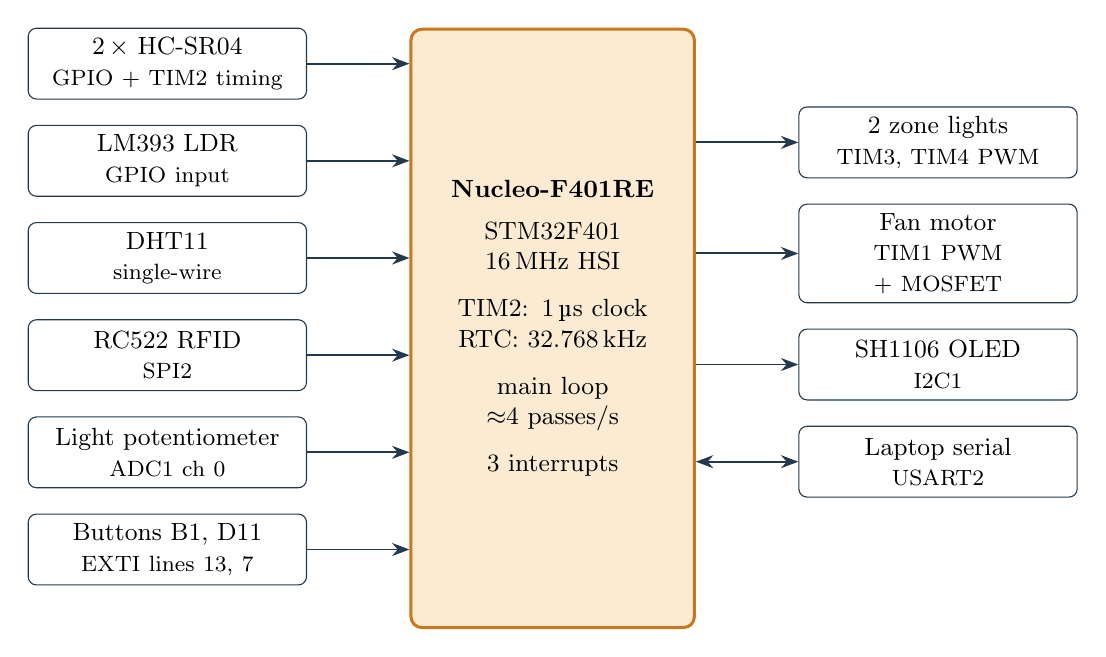
\begin{tikzpicture}[node distance=0.32cm and 1.3cm]
\node[hub,minimum width=3.6cm,minimum height=7.6cm,text width=3.3cm] (mcu) {\textbf{Nucleo-F401RE}\\[4pt]STM32F401\\16\,MHz HSI\\[6pt]TIM2: 1\,\textmu s clock\\RTC: 32.768\,kHz\\[6pt]main loop\\$\approx$4 passes/s\\[6pt]3 interrupts};
\node[blk,anchor=north east] (us) at ($(mcu.north west)+(-1.3,0)$) {2\,$\times$ HC-SR04\\\footnotesize GPIO + TIM2 timing};
\node[blk,below=of us] (ldr) {LM393 LDR\\\footnotesize GPIO input};
\node[blk,below=of ldr] (dht) {DHT11\\\footnotesize single-wire};
\node[blk,below=of dht] (rfid) {RC522 RFID\\\footnotesize SPI2};
\node[blk,below=of rfid] (pots) {Light potentiometer\\\footnotesize ADC1 ch 0};
\node[blk,below=of pots] (btn) {Buttons B1, D11\\\footnotesize EXTI lines 13, 7};
\node[blk,anchor=north west] (leds) at ($(mcu.north east)+(1.3,-1.0)$) {2 zone lights\\\footnotesize TIM3, TIM4 PWM};
\node[blk,below=of leds] (fan) {Fan motor\\\footnotesize TIM1 PWM + MOSFET};
\node[blk,below=of fan] (oled) {SH1106 OLED\\\footnotesize I2C1};
\node[blk,below=of oled] (pc) {Laptop serial\\\footnotesize USART2};
\foreach \n in {us,ldr,dht,rfid,pots,btn} \draw[arr] (\n.east) -- (\n.east -| mcu.west);
\foreach \n in {leds,fan,oled} \draw[arr] (\n.west -| mcu.east) -- (\n.west);
\draw[arr,{Stealth[length=2.2mm]}-{Stealth[length=2.2mm]}] (pc.west -| mcu.east) -- (pc.west);
\end{tikzpicture}
\end{document}
